% A pure minimalistic LaTeX-Beamer theme for everyone to use.
% Copyright (C) 2020 Kai Norman Clasen

% This program is free software: you can redistribute it and/or modify
% it under the terms of the GNU General Public License as published by
% the Free Software Foundation, either version 3 of the License, or
% (at your option) any later version.

% This program is distributed in the hope that it will be useful,
% but WITHOUT ANY WARRANTY; without even the implied warranty of
% MERCHANTABILITY or FITNESS FOR A PARTICULAR PURPOSE.  See the
% GNU General Public License for more details.

% You should have received a copy of the GNU General Public License
% along with this program.  If not, see <https://www.gnu.org/licenses/>.

% This file is part of beamerthemepureminimalistic.

% If problems/bugs are found or enhancements are desired, please contact
% me over: https://github.com/kai-tub/latex-beamer-pure-minimalistic

\documentclass[aspectratio=169]{beamer}
% should also look nice for the classic aspectratio
% of course, than the text has to be refitted
% \documentclass{beamer} 
\usepackage[utf8]{inputenc}
\usepackage[T1]{fontenc}
\usepackage{tikz}
\usetheme[showmaxslides]{pureminimalistic}

\usepackage[backend=biber, doi=false, maxbibnames=2, maxcitenames=2,%
            style=numeric, sorting=none, url=false, eprint=false]{biblatex}
\addbibresource{demo_bib.bib}
% this makes it possible to add backup slides, without counting them
\usepackage{appendixnumberbeamer}
\renewcommand{\appendixname}{\texorpdfstring{\translate{appendix}}{appendix}}

\usetheme{pureminimalistic}
\definecolor{textcolor}{RGB}{0, 0, 120}
\definecolor{title}{RGB}{0, 0, 0}
\definecolor{footercolor}{RGB}{133, 133, 133}
\definecolor{bg}{RGB}{255, 255, 255}
\definecolor{darkred}{RGB}{90,0,0}
\renewcommand{\beamertextcolor}{textcolor}
\renewcommand{\beamerbgcolor}{bg}
\renewcommand{\beamerfootertextcolor}{footercolor}
\renewcommand{\beamertitlecolor}{title}

\renewcommand{\logofooter}{}

\renewcommand{\logotitle}{
\begin{minipage}{0.7\linewidth}
\flushright
{\color{darkred} \LARGE
J\"{u}lich Summer School on\\
Fire Dynamics Modeling}
\end{minipage}
\hspace{0.25cm}
\begin{minipage}{0.25\linewidth}
\flushright
\includegraphics%
[width=\linewidth]{logos/cce_logo_standalone.png}
\end{minipage}
}

\renewcommand{\logoheader}{\includegraphics%
[width=.4\linewidth]{logos/cce_logo_standalone.png}}

% \renewcommand{\logoheader}{\includegraphics%
% [width=.6\linewidth]{logos/Juelich_1200.png}}

\renewcommand{\logofooter}{J\"{u}lich Summer School}

% if loaded after begin{document} a warning will appear: "pdfauthor already used"
\title[BlenderFDS]{Introduction to BlenderFDS}
\author{Emanuele Gissi}
\institute{Corpo nazionale dei Vigili del fuoco, Italy} 
\date{\today}

\begin{document}
% has to be loaded outside of a frame to work!
\maketitle

% For longer table of contents, I find it cleaner to
% use no footline.
\begin{frame}[plain, noframenumbering]{Outline}
  \tableofcontents
\end{frame}

\section{Objectives and rules}
\begin{frame}[fragile]{Learning objectives}
  \begin{vfilleditems}
    \item<1-> Get \textit{curious} about BlenderFDS approach to writing FDS cases,
        \linebreak and learn how to prepare a simple case.
    \item<2-> \emph{[If we got time]} Take a stroll to the Golden Gate in California,
        \linebreak and get to know about the existence of qgis2fds.
  \end{vfilleditems}
\end{frame}

\begin{frame}[fragile]{House rules}
    \begin{vfilleditems}
        \item<1-> Be interactive: $\nexists$ stupid questions, so stop me and ask.
        \item<2-> Play hard, break your computer.
        \item<3-> \emph{[Never forget]} Fire safety is not just compliance to your           country's regulations, but \emph{effective} life, property, and environment           protection.
    \end{vfilleditems}
\end{frame}

\section{Blender + FDS = BlenderFDS}
\begin{frame}[fragile]{Blender + FDS = BlenderFDS}
    \begin{vfilleditems}
        \item<1-> Blender, \url{http://blender.org}
            {\small \linebreak a free and open source 3D creation suite with a huge worldwide Community.
            \linebreak It supports the entirety of the 3D pipeline from modelling to visualisation.$\nearrow$}
        \item<2-> FDS, \url{https://pages.nist.gov/fds-smv/}
            {\small \linebreak \emph{[you should know it by now!]}}
        \item<3-> BlenderFDS, \url{http://blenderfds.org}
            {\small \linebreak a tool that helps you building complex FDS models faster,
            \linebreak because it eases geometric data entry with powerful 3D editing tools.}
    \end{vfilleditems}  
\end{frame}

\begin{frame}[fragile]{BlenderFDS}
    \begin{vfilleditems}
        \item<1-> Developed in Python as an addon to Blender, since 2009.
        \item<2-> Free, open source, and multi platform
            {\small \linebreak Linux, MacOS, and MS Windows versions.}
        \item<3-> Importing/exporting
            {\small \linebreak FDS cases to/from Blender files.
            \linebreak Geometries from your preferred CAD/BIM tools.}
        \item<4-> \emph{Full control} over all the input parameters,
            {\small \linebreak FDS complexity and flexibility are not hidden from your eyes. }
    \end{vfilleditems}  
\end{frame}

\begin{frame}[fragile]{BlenderFDS resources}
    The main entry point is its website: \url{http://blenderfds.org}:
    \begin{vfilleditems}
        \item Discussion group.
        \item Documentation.
        \item GitHub code repository
        \item Issue tracker.
        \item Verification suite.
    \end{vfilleditems}
\end{frame}

\section{Let's use BlenderFDS}
\begin{frame}[fragile]{}
  \centering
  \vfill
  {\fontsize{20}{50}\selectfont Let's use BlenderFDS}
  \linebreak
  {\fontsize{40}{50}\selectfont together!}
  \centering
  \vfill
  
\includegraphics[width=.65\linewidth]{images/people.jpg}
  \vfill
\end{frame}

\begin{frame}[fragile]{What we learned so far: \linebreak running BlenderFDS}
    \begin{vfilleditems}
        \item Install the BlenderFDS addon in Blender, beware the right version!
        \item Set the Preferences: default case and simplified UI.
        \item Save the blend file, and set the FDS case directory.
        \item Run the FDS case in FDS and open Smokeview.
        \item Import another FDS case as a new Blender Scene.
    \end{vfilleditems}
\end{frame}

\begin{frame}[fragile]{What we learned so far: Blender Editors}
  \centering
  \vfill
  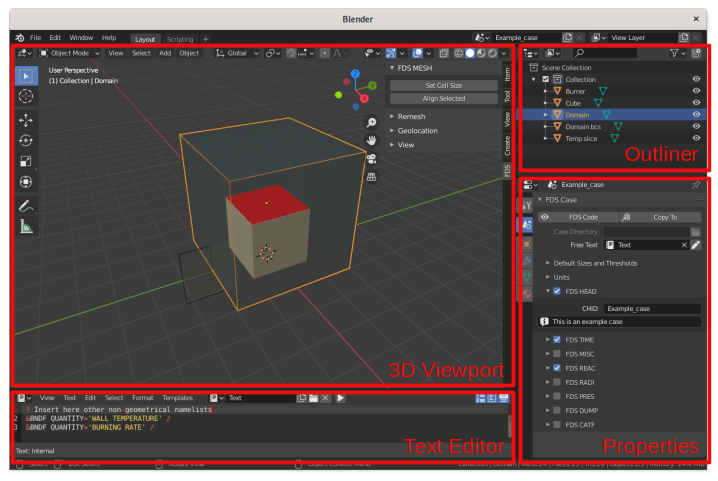
\includegraphics[width=.65\linewidth]{images/bf_editors.png}
  \vfill
\end{frame}

\begin{frame}[fragile]{What we learned so far: \linebreak Blender Modes and keyboard shortcuts}
    \begin{vfilleditems}
        \item Object Mode [tab]
        {\small \linebreak transform the Object
        \linebreak with grab [G], rotate [R], and scale [S],
        \linebreak along the axis [X] [Y] [Z].}
        \item Edit Mode [tab]
        {\small \linebreak create and modify its shape,
        \linebreak by selecting vertices [1], edges [2], faces [3]
        \linebreak and then grab [G], rotate [R], scale [S], extrude [E], ...}
    \end{vfilleditems}
\end{frame}

\begin{frame}[fragile]{What we learned so far: \linebreak Blender Datablocks in the Outliner}
    
    \tikzset{every picture/.style={line width=0.75pt}} %set default line width to 0.75pt        
    
    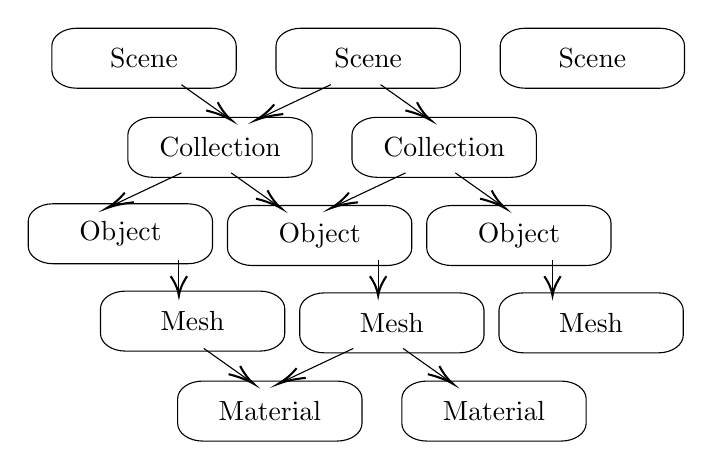
\begin{tikzpicture}[x=0.75pt,y=0.75pt,yscale=-.85,xscale=1.2]
    %uncomment if require: \path (0,300); %set diagram left start at 0, and has height of 300
    
    %Straight Lines [id:da5647906959220583] 
    \draw    (130,40.5) -- (101.66,59.39) ;
    \draw [shift={(100,60.5)}, rotate = 326.31] [color={rgb, 255:red, 0; green, 0; blue, 0 }  ][line width=0.75]    (10.93,-3.29) .. controls (6.95,-1.4) and (3.31,-0.3) .. (0,0) .. controls (3.31,0.3) and (6.95,1.4) .. (10.93,3.29)   ;
    %Straight Lines [id:da30636214697744757] 
    \draw    (70,40.5) -- (88.59,59.09) ;
    \draw [shift={(90,60.5)}, rotate = 225] [color={rgb, 255:red, 0; green, 0; blue, 0 }  ][line width=0.75]    (10.93,-3.29) .. controls (6.95,-1.4) and (3.31,-0.3) .. (0,0) .. controls (3.31,0.3) and (6.95,1.4) .. (10.93,3.29)   ;
    %Straight Lines [id:da8842309995802216] 
    \draw    (150,40.5) -- (155.7,46.2) -- (168.59,59.09) ;
    \draw [shift={(170,60.5)}, rotate = 225] [color={rgb, 255:red, 0; green, 0; blue, 0 }  ][line width=0.75]    (10.93,-3.29) .. controls (6.95,-1.4) and (3.31,-0.3) .. (0,0) .. controls (3.31,0.3) and (6.95,1.4) .. (10.93,3.29)   ;
    %Straight Lines [id:da17256325488418645] 
    \draw    (70,90.5) -- (41.66,109.39) ;
    \draw [shift={(40,110.5)}, rotate = 326.31] [color={rgb, 255:red, 0; green, 0; blue, 0 }  ][line width=0.75]    (10.93,-3.29) .. controls (6.95,-1.4) and (3.31,-0.3) .. (0,0) .. controls (3.31,0.3) and (6.95,1.4) .. (10.93,3.29)   ;
    %Straight Lines [id:da9181217129726917] 
    \draw    (90,90.5) -- (95.7,96.2) -- (108.59,109.09) ;
    \draw [shift={(110,110.5)}, rotate = 225] [color={rgb, 255:red, 0; green, 0; blue, 0 }  ][line width=0.75]    (10.93,-3.29) .. controls (6.95,-1.4) and (3.31,-0.3) .. (0,0) .. controls (3.31,0.3) and (6.95,1.4) .. (10.93,3.29)   ;
    %Straight Lines [id:da9906853710907666] 
    \draw    (160,90.5) -- (131.66,109.39) ;
    \draw [shift={(130,110.5)}, rotate = 326.31] [color={rgb, 255:red, 0; green, 0; blue, 0 }  ][line width=0.75]    (10.93,-3.29) .. controls (6.95,-1.4) and (3.31,-0.3) .. (0,0) .. controls (3.31,0.3) and (6.95,1.4) .. (10.93,3.29)   ;
    %Straight Lines [id:da4826829941132442] 
    \draw    (180,90.5) -- (185.7,96.2) -- (198.59,109.09) ;
    \draw [shift={(200,110.5)}, rotate = 225] [color={rgb, 255:red, 0; green, 0; blue, 0 }  ][line width=0.75]    (10.93,-3.29) .. controls (6.95,-1.4) and (3.31,-0.3) .. (0,0) .. controls (3.31,0.3) and (6.95,1.4) .. (10.93,3.29)   ;
    %Straight Lines [id:da9264135859659843] 
    \draw    (149,140) -- (149,150) -- (149,158) ;
    \draw [shift={(149,160)}, rotate = 270] [color={rgb, 255:red, 0; green, 0; blue, 0 }  ][line width=0.75]    (10.93,-3.29) .. controls (6.95,-1.4) and (3.31,-0.3) .. (0,0) .. controls (3.31,0.3) and (6.95,1.4) .. (10.93,3.29)   ;
    %Straight Lines [id:da21061594939017536] 
    \draw    (69,140) -- (69,150) -- (69,158) ;
    \draw [shift={(69,160)}, rotate = 270] [color={rgb, 255:red, 0; green, 0; blue, 0 }  ][line width=0.75]    (10.93,-3.29) .. controls (6.95,-1.4) and (3.31,-0.3) .. (0,0) .. controls (3.31,0.3) and (6.95,1.4) .. (10.93,3.29)   ;
    %Straight Lines [id:da8478884705342151] 
    \draw    (219,140) -- (219,150) -- (219,158) ;
    \draw [shift={(219,160)}, rotate = 270] [color={rgb, 255:red, 0; green, 0; blue, 0 }  ][line width=0.75]    (10.93,-3.29) .. controls (6.95,-1.4) and (3.31,-0.3) .. (0,0) .. controls (3.31,0.3) and (6.95,1.4) .. (10.93,3.29)   ;
    %Straight Lines [id:da1910023521634565] 
    \draw    (139,190) -- (110.66,208.89) ;
    \draw [shift={(109,210)}, rotate = 326.31] [color={rgb, 255:red, 0; green, 0; blue, 0 }  ][line width=0.75]    (10.93,-3.29) .. controls (6.95,-1.4) and (3.31,-0.3) .. (0,0) .. controls (3.31,0.3) and (6.95,1.4) .. (10.93,3.29)   ;
    %Straight Lines [id:da7833026803205954] 
    \draw    (159,190) -- (164.7,195.7) -- (177.59,208.59) ;
    \draw [shift={(179,210)}, rotate = 225] [color={rgb, 255:red, 0; green, 0; blue, 0 }  ][line width=0.75]    (10.93,-3.29) .. controls (6.95,-1.4) and (3.31,-0.3) .. (0,0) .. controls (3.31,0.3) and (6.95,1.4) .. (10.93,3.29)   ;
    %Straight Lines [id:da5811344891085861] 
    \draw    (79,190) -- (84.7,195.7) -- (97.59,208.59) ;
    \draw [shift={(99,210)}, rotate = 225] [color={rgb, 255:red, 0; green, 0; blue, 0 }  ][line width=0.75]    (10.93,-3.29) .. controls (6.95,-1.4) and (3.31,-0.3) .. (0,0) .. controls (3.31,0.3) and (6.95,1.4) .. (10.93,3.29)   ;
    
    
    % Text Node
    \draw    (18,18.5) .. controls (18,12.98) and (22.48,8.5) .. (28,8.5) -- (82,8.5) .. controls (87.52,8.5) and (92,12.98) .. (92,18.5) -- (92,32.5) .. controls (92,38.02) and (87.52,42.5) .. (82,42.5) -- (28,42.5) .. controls (22.48,42.5) and (18,38.02) .. (18,32.5) -- cycle  ;
    \draw (55,25.5) node   [align=left] {\begin{minipage}[lt]{47.6pt}\setlength\topsep{0pt}
    \begin{center}
    Scene
    \end{center}
    
    \end{minipage}};
    % Text Node
    \draw    (108,18.5) .. controls (108,12.98) and (112.48,8.5) .. (118,8.5) -- (172,8.5) .. controls (177.52,8.5) and (182,12.98) .. (182,18.5) -- (182,32.5) .. controls (182,38.02) and (177.52,42.5) .. (172,42.5) -- (118,42.5) .. controls (112.48,42.5) and (108,38.02) .. (108,32.5) -- cycle  ;
    \draw (145,25.5) node   [align=left] {\begin{minipage}[lt]{47.6pt}\setlength\topsep{0pt}
    \begin{center}
    Scene
    \end{center}
    
    \end{minipage}};
    % Text Node
    \draw    (198,18.5) .. controls (198,12.98) and (202.48,8.5) .. (208,8.5) -- (262,8.5) .. controls (267.52,8.5) and (272,12.98) .. (272,18.5) -- (272,32.5) .. controls (272,38.02) and (267.52,42.5) .. (262,42.5) -- (208,42.5) .. controls (202.48,42.5) and (198,38.02) .. (198,32.5) -- cycle  ;
    \draw (235,25.5) node   [align=left] {\begin{minipage}[lt]{47.6pt}\setlength\topsep{0pt}
    \begin{center}
    Scene
    \end{center}
    
    \end{minipage}};
    % Text Node
    \draw    (48.5,69) .. controls (48.5,63.48) and (52.98,59) .. (58.5,59) -- (112.5,59) .. controls (118.02,59) and (122.5,63.48) .. (122.5,69) -- (122.5,83) .. controls (122.5,88.52) and (118.02,93) .. (112.5,93) -- (58.5,93) .. controls (52.98,93) and (48.5,88.52) .. (48.5,83) -- cycle  ;
    \draw (85.5,76) node   [align=left] {\begin{minipage}[lt]{55pt}\setlength\topsep{0pt}
    \begin{center}
    Collection
    \end{center}
    
    \end{minipage}};
    % Text Node
    \draw    (138.5,69) .. controls (138.5,63.48) and (142.98,59) .. (148.5,59) -- (202.5,59) .. controls (208.02,59) and (212.5,63.48) .. (212.5,69) -- (212.5,83) .. controls (212.5,88.52) and (208.02,93) .. (202.5,93) -- (148.5,93) .. controls (142.98,93) and (138.5,88.52) .. (138.5,83) -- cycle  ;
    \draw (175.5,76) node   [align=left] {\begin{minipage}[lt]{55pt}\setlength\topsep{0pt}
    \begin{center}
    Collection
    \end{center}
    
    \end{minipage}};
    % Text Node
    \draw    (8.5,118) .. controls (8.5,112.48) and (12.98,108) .. (18.5,108) -- (72.5,108) .. controls (78.02,108) and (82.5,112.48) .. (82.5,118) -- (82.5,132) .. controls (82.5,137.52) and (78.02,142) .. (72.5,142) -- (18.5,142) .. controls (12.98,142) and (8.5,137.52) .. (8.5,132) -- cycle  ;
    \draw (45.5,125) node   [align=left] {\begin{minipage}[lt]{47.6pt}\setlength\topsep{0pt}
    \begin{center}
    Object
    \end{center}
    
    \end{minipage}};
    % Text Node
    \draw    (88.5,119) .. controls (88.5,113.48) and (92.98,109) .. (98.5,109) -- (152.5,109) .. controls (158.02,109) and (162.5,113.48) .. (162.5,119) -- (162.5,133) .. controls (162.5,138.52) and (158.02,143) .. (152.5,143) -- (98.5,143) .. controls (92.98,143) and (88.5,138.52) .. (88.5,133) -- cycle  ;
    \draw (125.5,126) node   [align=left] {\begin{minipage}[lt]{47.6pt}\setlength\topsep{0pt}
    \begin{center}
    Object
    \end{center}
    
    \end{minipage}};
    % Text Node
    \draw    (168.5,119) .. controls (168.5,113.48) and (172.98,109) .. (178.5,109) -- (232.5,109) .. controls (238.02,109) and (242.5,113.48) .. (242.5,119) -- (242.5,133) .. controls (242.5,138.52) and (238.02,143) .. (232.5,143) -- (178.5,143) .. controls (172.98,143) and (168.5,138.52) .. (168.5,133) -- cycle  ;
    \draw (205.5,126) node   [align=left] {\begin{minipage}[lt]{47.6pt}\setlength\topsep{0pt}
    \begin{center}
    Object
    \end{center}
    
    \end{minipage}};
    % Text Node
    \draw    (37.5,167.5) .. controls (37.5,161.98) and (41.98,157.5) .. (47.5,157.5) -- (101.5,157.5) .. controls (107.02,157.5) and (111.5,161.98) .. (111.5,167.5) -- (111.5,181.5) .. controls (111.5,187.02) and (107.02,191.5) .. (101.5,191.5) -- (47.5,191.5) .. controls (41.98,191.5) and (37.5,187.02) .. (37.5,181.5) -- cycle  ;
    \draw (74.5,174.5) node   [align=left] {\begin{minipage}[lt]{47.6pt}\setlength\topsep{0pt}
    \begin{center}
    Mesh
    \end{center}
    
    \end{minipage}};
    % Text Node
    \draw    (117.5,168.5) .. controls (117.5,162.98) and (121.98,158.5) .. (127.5,158.5) -- (181.5,158.5) .. controls (187.02,158.5) and (191.5,162.98) .. (191.5,168.5) -- (191.5,182.5) .. controls (191.5,188.02) and (187.02,192.5) .. (181.5,192.5) -- (127.5,192.5) .. controls (121.98,192.5) and (117.5,188.02) .. (117.5,182.5) -- cycle  ;
    \draw (154.5,175.5) node   [align=left] {\begin{minipage}[lt]{47.6pt}\setlength\topsep{0pt}
    \begin{center}
    Mesh
    \end{center}
    
    \end{minipage}};
    % Text Node
    \draw    (197.5,168.5) .. controls (197.5,162.98) and (201.98,158.5) .. (207.5,158.5) -- (261.5,158.5) .. controls (267.02,158.5) and (271.5,162.98) .. (271.5,168.5) -- (271.5,182.5) .. controls (271.5,188.02) and (267.02,192.5) .. (261.5,192.5) -- (207.5,192.5) .. controls (201.98,192.5) and (197.5,188.02) .. (197.5,182.5) -- cycle  ;
    \draw (234.5,175.5) node   [align=left] {\begin{minipage}[lt]{47.6pt}\setlength\topsep{0pt}
    \begin{center}
    Mesh
    \end{center}
    
    \end{minipage}};
    % Text Node
    \draw    (68.5,218.5) .. controls (68.5,212.98) and (72.98,208.5) .. (78.5,208.5) -- (132.5,208.5) .. controls (138.02,208.5) and (142.5,212.98) .. (142.5,218.5) -- (142.5,232.5) .. controls (142.5,238.02) and (138.02,242.5) .. (132.5,242.5) -- (78.5,242.5) .. controls (72.98,242.5) and (68.5,238.02) .. (68.5,232.5) -- cycle  ;
    \draw (105.5,225.5) node   [align=left] {\begin{minipage}[lt]{47.6pt}\setlength\topsep{0pt}
    \begin{center}
    Material
    \end{center}
    
    \end{minipage}};
    % Text Node
    \draw    (158.5,218.5) .. controls (158.5,212.98) and (162.98,208.5) .. (168.5,208.5) -- (222.5,208.5) .. controls (228.02,208.5) and (232.5,212.98) .. (232.5,218.5) -- (232.5,232.5) .. controls (232.5,238.02) and (228.02,242.5) .. (222.5,242.5) -- (168.5,242.5) .. controls (162.98,242.5) and (158.5,238.02) .. (158.5,232.5) -- cycle  ;
    \draw (195.5,225.5) node   [align=left] {\begin{minipage}[lt]{47.6pt}\setlength\topsep{0pt}
    \begin{center}
    Material
    \end{center}
    
    \end{minipage}};
    
    \end{tikzpicture}

\end{frame}

\section{Let's build a simple FDS case from scratch}
\begin{frame}[fragile]{}
  \centering
  \vfill
  {\fontsize{20}{50}\selectfont We are ready to build \linebreak a simple FDS case from scratch}
  \vfill
\end{frame}

\begin{frame}[fragile]{A room with two burners}
  \vfill
  {\tiny Feel free to choose the missing data!}
  \centering
  \vfill
  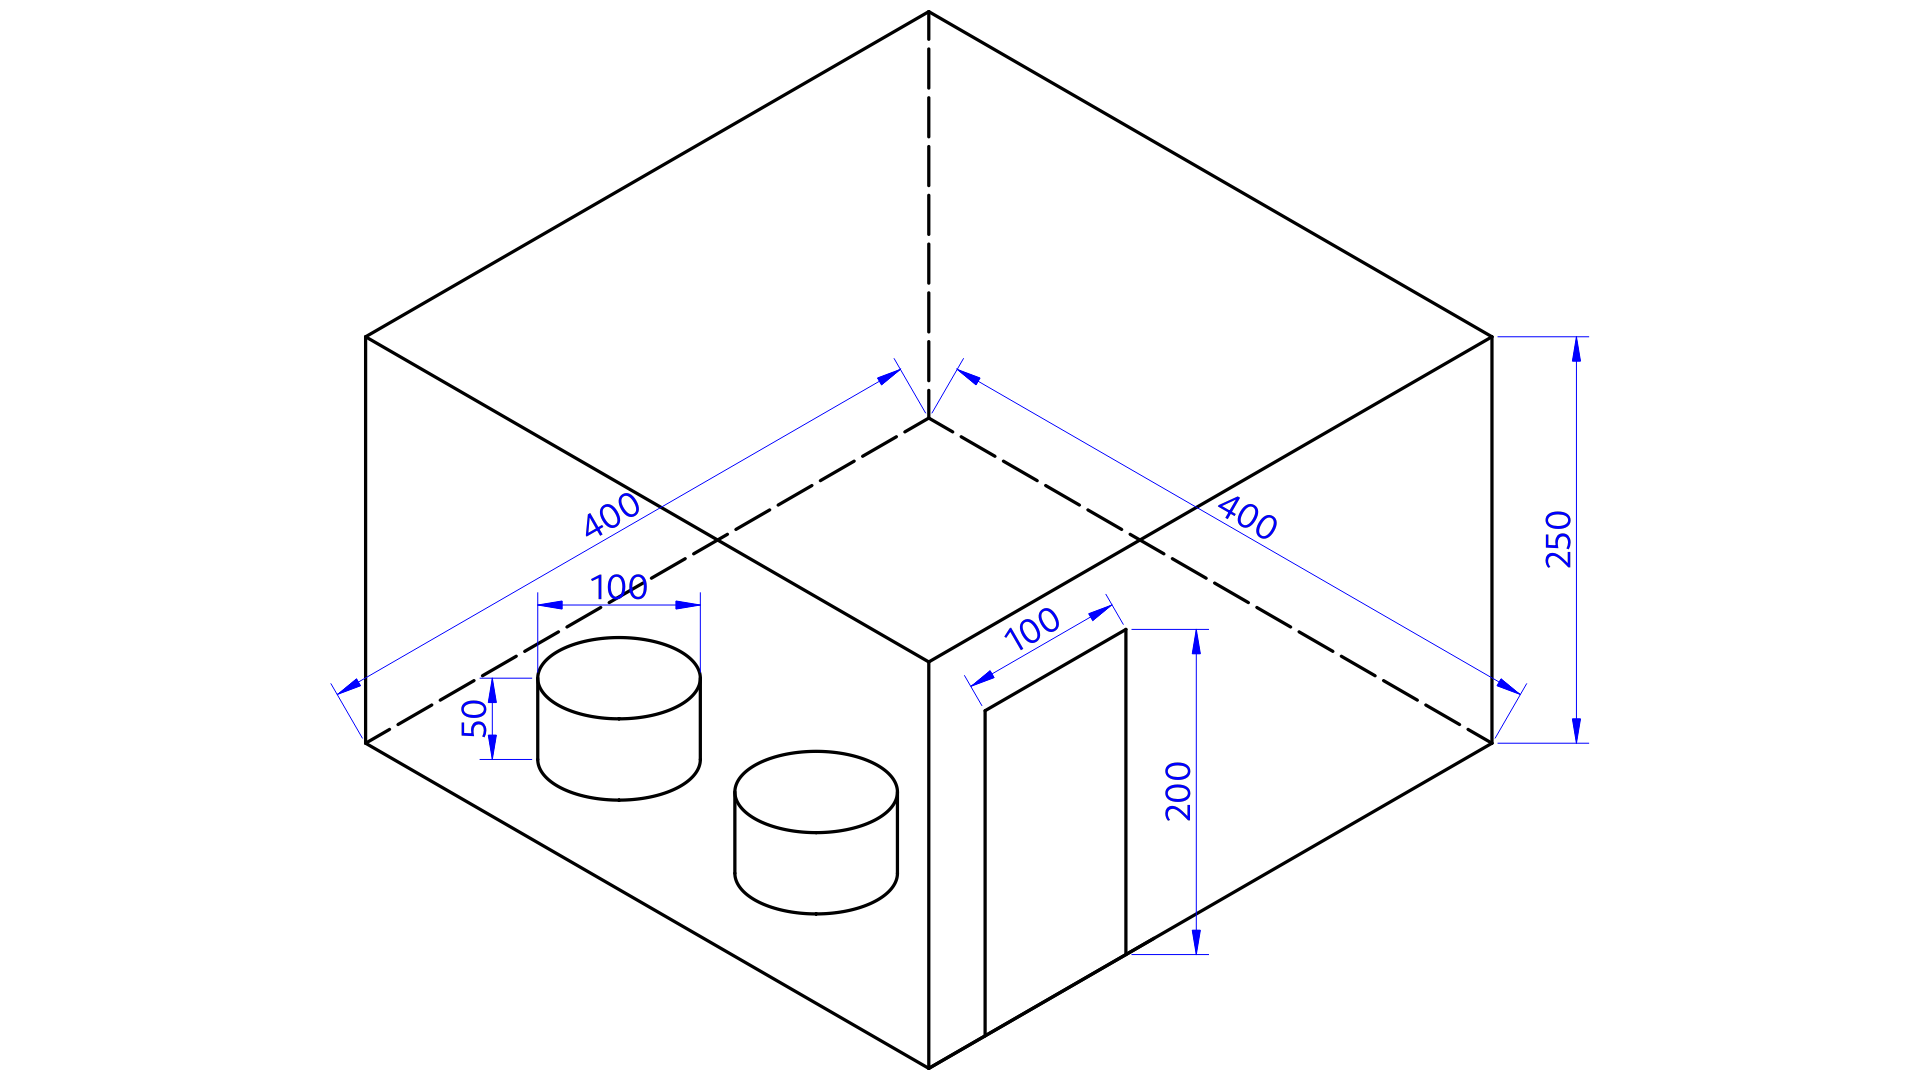
\includegraphics[width=.7\linewidth]{images/case.png}
  \vfill
\end{frame}

\begin{frame}[fragile]{}
  \centering
  \vfill
  {\fontsize{20}{50}\selectfont Let's build a simple FDS case}
  \linebreak
  {\fontsize{40}{50}\selectfont together!}
  \centering
  \vfill
  
\includegraphics[width=.65\linewidth]{images/people.jpg}
  \vfill
\end{frame}

\begin{frame}[fragile]{What we learned so far: \linebreak FDS $\leftrightarrow$ Blender}
    \begin{vfilleditems}
        \item<1-> FDS case $\leftrightarrow$ Blender Scene
        {\small \linebreak HEAD, TIME, MISC, REAC, RADI, PRES, DUMP}
        \item<2-> Geometric FDS namelist $\leftrightarrow$ Blender Object
        {\small \linebreak MESH, OBST, VENT, HOLE, GEOM, DEVC, SLCF, ...}
        \item<3-> FDS boundary condition $\leftrightarrow$ Blender Material
        {\small \linebreak SURF}
        \item<4-> Other FDS namelists $\leftrightarrow$ Blender Text, inserted verbatim
        {\small \linebreak MATL, PART, BNDF, ...}
    \end{vfilleditems}
\end{frame}

\begin{frame}[fragile]{What we learned so far:
\linebreak Blender geometry $\rightarrow$ FDS notation}
    \begin{figure}[H]
        \centering
        \begin{columns}[T]
            \begin{column}{.3\linewidth}
                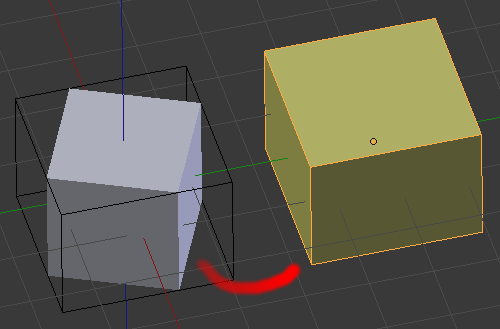
\includegraphics[width=\linewidth]{images/T_BBOX.png}
                \caption{Bounding Box $\rightarrow$ XB}
            \end{column}
            \begin{column}{.3\linewidth}
                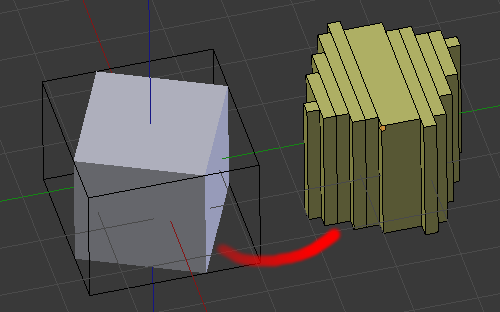
\includegraphics[width=\linewidth]{images/T_VOXELS.png}
                \caption{Voxels $\rightarrow$ XBs}
            \end{column}
            \begin{column}{.3\linewidth}
                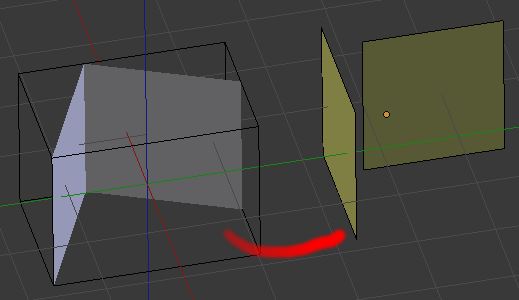
\includegraphics[width=\linewidth]{images/T_FACES.png}
                \caption{Faces $\rightarrow$ XBs}
            \end{column}
        \end{columns}
    \end{figure}
\end{frame}

\begin{frame}[fragile]{What we learned so far:
\linebreak Blender geometry $\rightarrow$ FDS notation}
    \begin{vfilleditems}
        \item Bounding Box, Voxels, Faces, Pixels, Edges $\rightarrow$ XBs
        \item Vertices, Center $\rightarrow$ XYZs
        \item Planes $\rightarrow$ PBXs, PBYs, PBZs
        \item Blender Mesh (triangulated surface) $\rightarrow$ GEOM bingeom file
    \end{vfilleditems}
\end{frame}

\begin{frame}[fragile]{A room with two burners, in BlenderFDS}
  \centering
  \vfill
  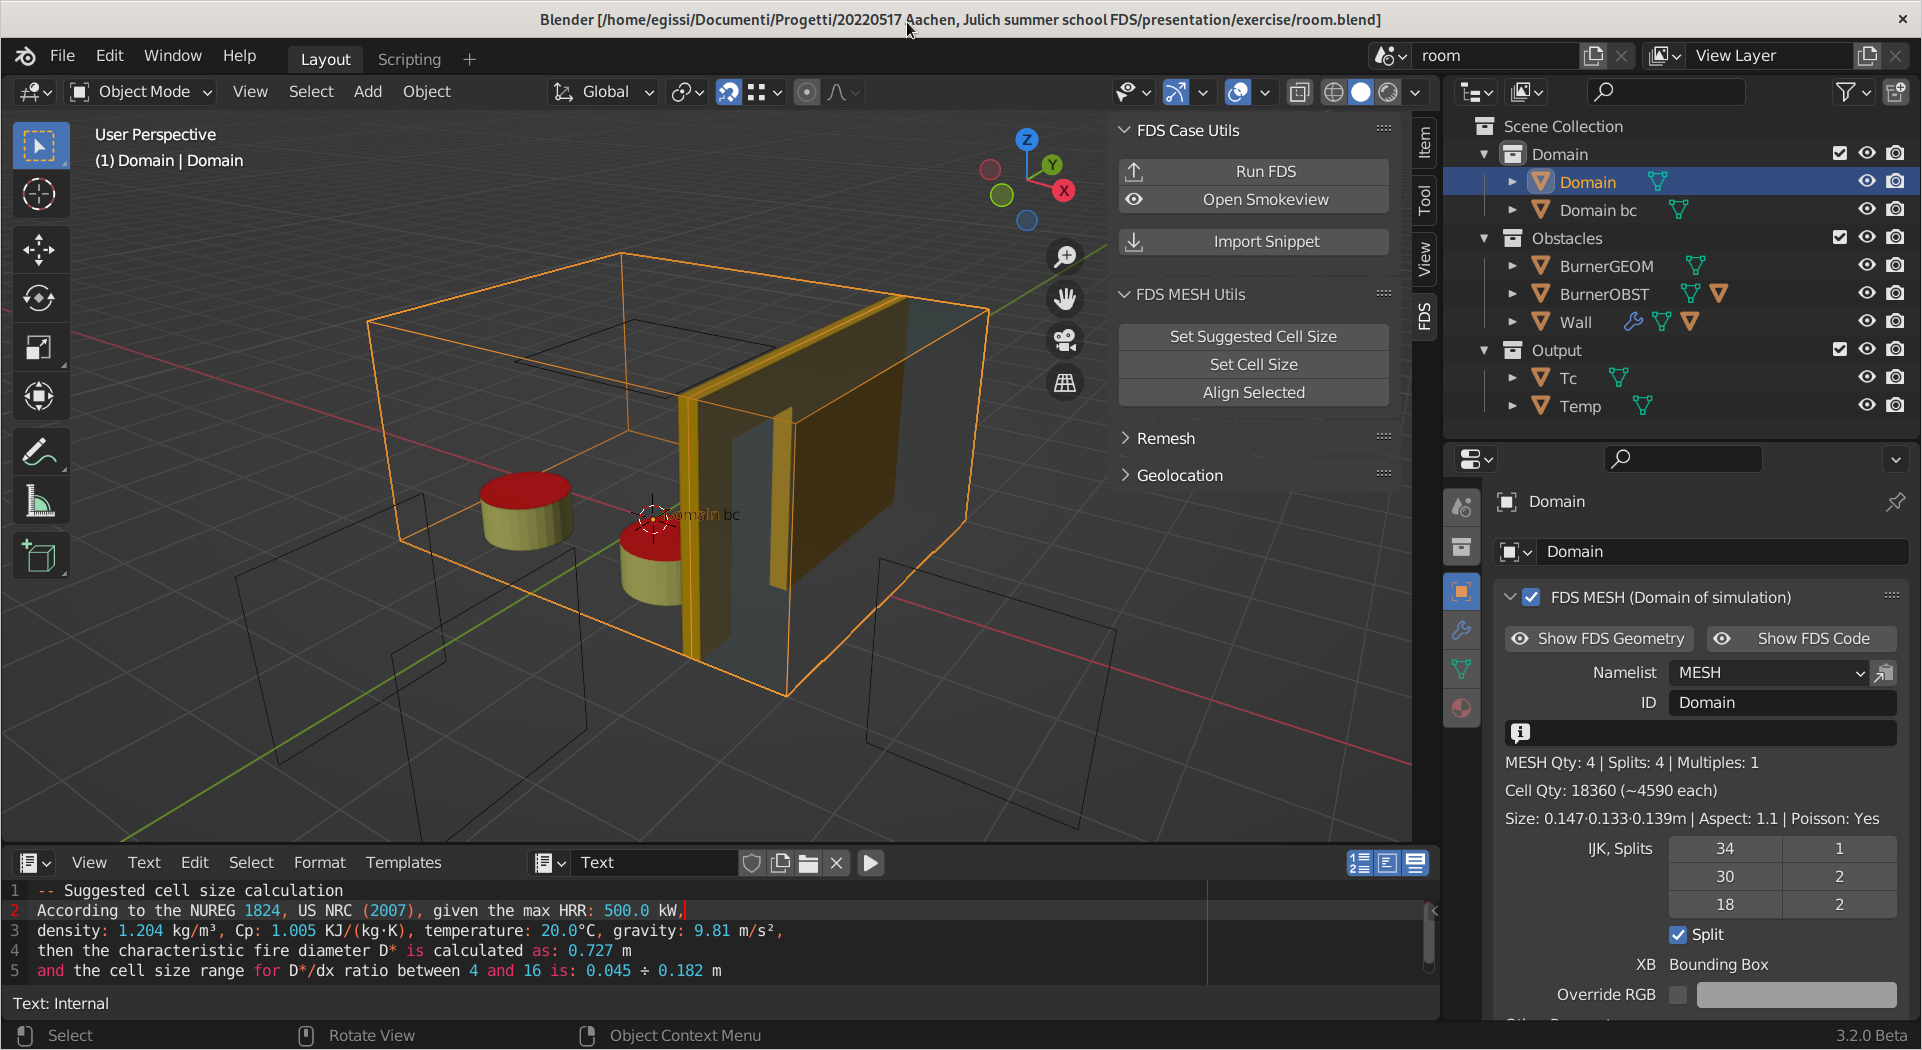
\includegraphics[width=.75\linewidth]{images/blend_case.png}
  \vfill
\end{frame}

\begin{frame}[fragile]{A room with two burners, in Smokeview}
  \centering
  \vfill
  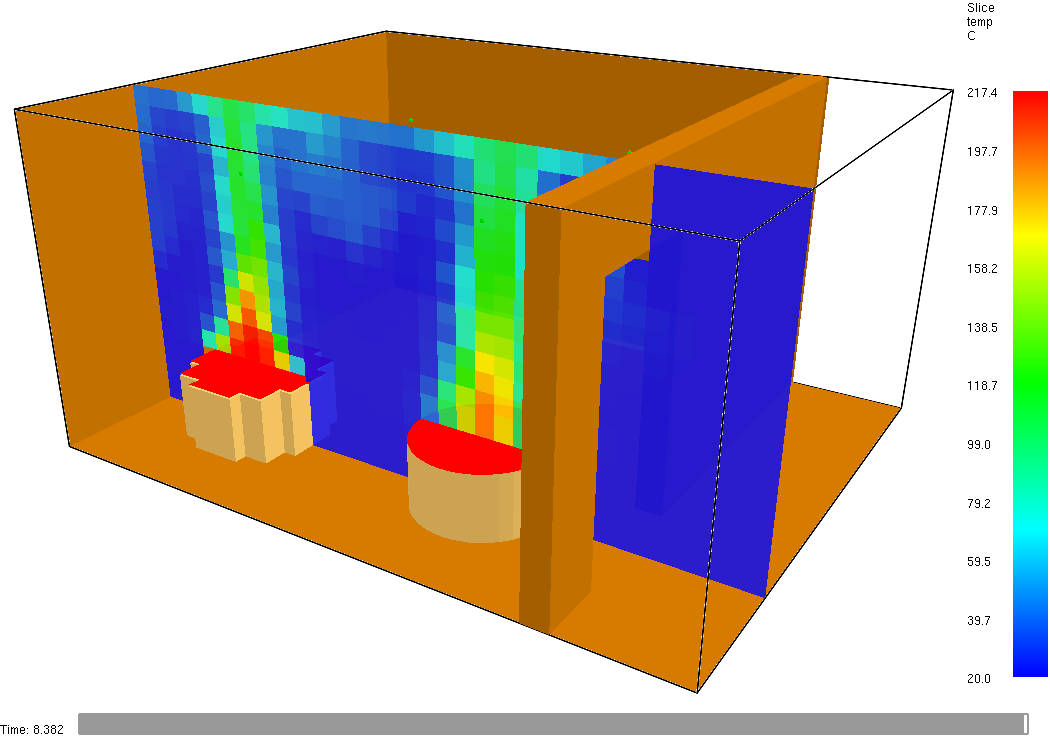
\includegraphics[width=.6\linewidth]{images/smv_case.png}
  \vfill
\end{frame}

\begin{frame}[fragile]{}
  \centering
  \vfill
  {\fontsize{20}{50}\selectfont Any further question?}
  \linebreak
  {\fontsize{40}{50}\selectfont Thank you!}
  \linebreak
  {\fontsize{15}{50}\selectfont emanuele.gissi@vigilfuoco.it}
  \centering
  \vfill
  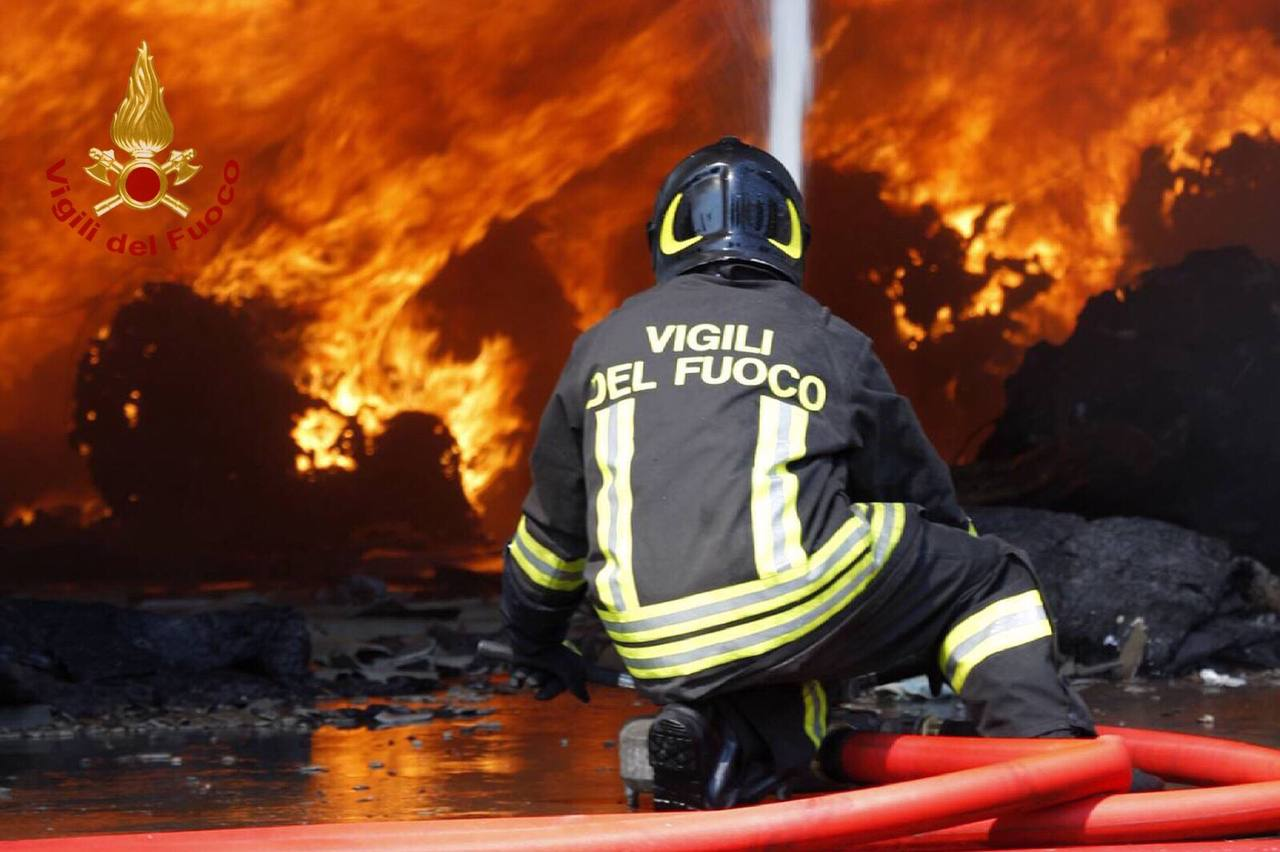
\includegraphics[width=.35\linewidth]{images/vigilifuoco.jpeg}
  \vfill
\end{frame}

\end{document}

    



